\chapter{Hand Features and Representations}

Different hand feature representation and encoding methods are compared. The
hand features can be extracted from either color, depth or both images. 
\begin{figure}[h]
  \centering
  \subfigure[Color images] {
	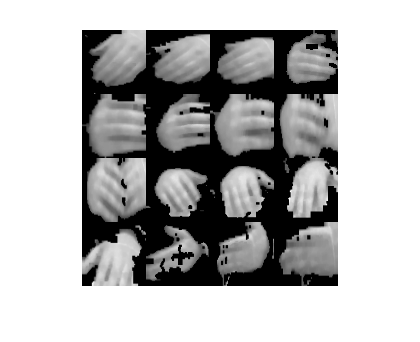
\includegraphics[width=0.45\textwidth]{figures/color_hand.png} 
  }
  \subfigure[Depth images] {
  	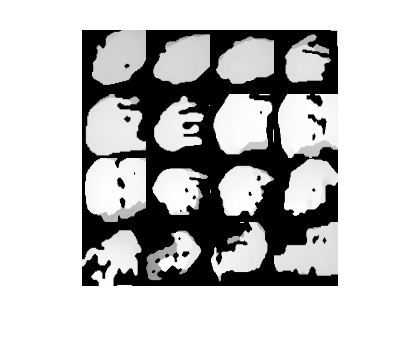
\includegraphics[width=0.45\textwidth]{figures/depth_hand.png}
  }
  \caption{$64\times64$ pixel raw image patches of hands.} \label{fig:hand}
\end{figure}

\begin{figure}[h]
\centering
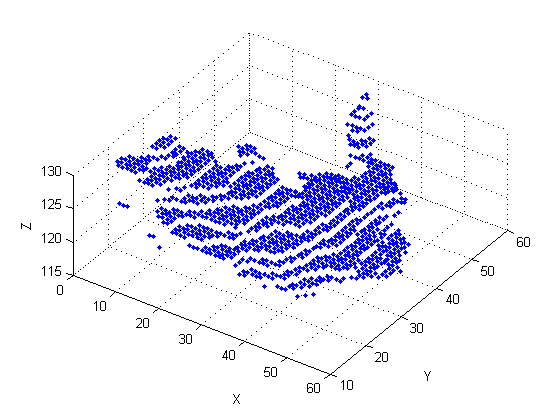
\includegraphics{figures/hand3d.png}
\caption{View of quantized depth data of a hand in 3D.}
\end{figure}

\section{Histogram of Oriented Gradients}
For each pixel, the magnitude of gradient is 
\begin{align*}
m = \sqrt{dx^2 + dy^2}
\end{align*}

If an image $I$ has dimensions $m\times n$, the size of the computed feature
vector $H$ is $(m/\text{cell\_size} - 2) \times (n/\text{cell\_size} - 2)
\times \text{num\_bin}$.

\begin{figure}[h]
  \centering
  \subfigure[Color] {
  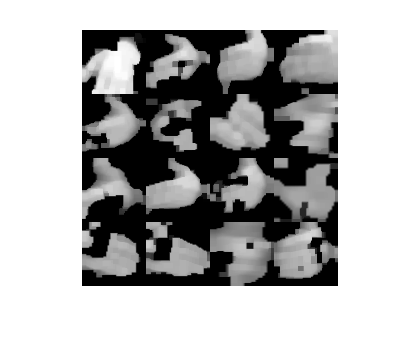
\includegraphics[width=0.45\textwidth]{figures/color_denoised_5.png} 
  }
  \subfigure[Depth] {
    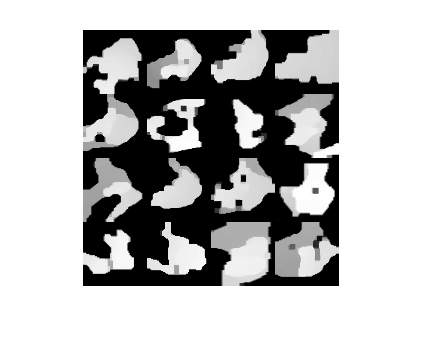
\includegraphics[width=0.45\textwidth]{figures/depth_denoised_5.png}
  }
  \subfigure[Color HOG] {
  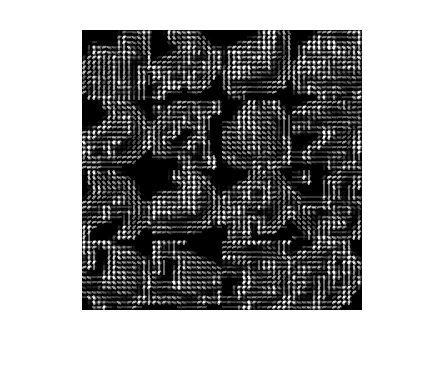
\includegraphics[width=0.45\textwidth]{figures/color_hog.png} }
  \subfigure[Depth HOG] {
    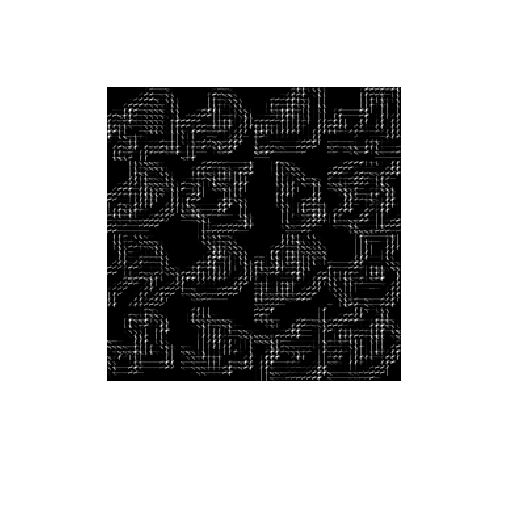
\includegraphics[trim={0cm 1.5cm 0cm 0cm},
  clip, width=0.5\textwidth]{figures/depth_hog.png}
  }
  \caption{$64\times64$ pixel image patches of hands.} \label{fig:hand}
\end{figure}

\section{Hand Feature Extraction}
We use both the Kinect and the Xsens data from the ChAirGest corpus~\cite{Ruffieux2013} to
extract hand motion feature vectors for gesture modeling.
It is relatively easy to obtain features from the Xsens data. We choose to use linear
acceleration (x, y, z), angular velocity (x, y, z) and Euler orientation (yaw, pitch, roll)
from the Xsens unit on the hand to form a 9-dimensional feature vector $\underline{x}_t^{\text{xsens}}$
for every time frame $t$.
From the Kinect sensor, we extract the position of the gesturing hand in (x, y, z) relative to
the shoulder center joint to
form a 3-dimensional vector $\underline{x}_t^{\text{kinect}}$. Combining the two, we
have a 12-dimensional feature vector $\underline{x}_t = [\underline{x}^\text{kinect}_t, \underline{x}^\text{xsens}_t]$.

Using temporal smoothing on the raw feature data does not necessarily improve
the results if we want to detect the gesture as soon as possible because it
introduces delay.

We use the Kinect skeleton tracking result for the shoulder center joint position,
but do not use it for the hand position because
it is not accurate when the hands are close to the body or when the hands are moving fast.
We developed an improved method for hand tracking based on gesture salience using both
RGB and depth data.

\section{SVM for hand pose classification}
SVM for unbalanced data. \cite{ben2010}
If we ignore the  fact that the data is unbalanced, the resultant classifier
will favor the majority class, in this case the ``other'' category. To take this
into account, we can assign different misclassification (SVM soft-margin
constants) to each class. If $n_1$ and $n_2$ are the number of examples in two
classes, 

\begin{align}
\frac{C_+}{C_-} = \frac{n_-}{n_+}
\end{align}

\begin{figure}
\centering
\subfigure[]{
  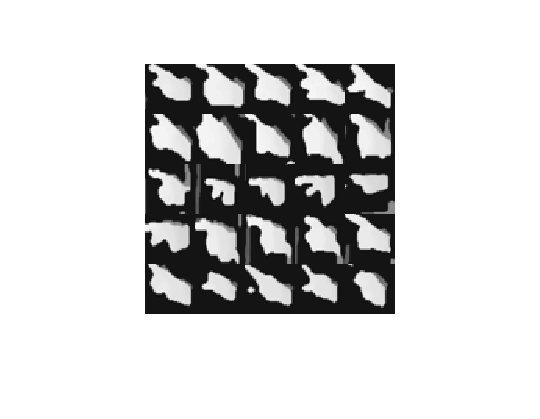
\includegraphics[width=0.5\linewidth,
  trim={0cm 1cm 0cm 0cm}, clip]{figures/point_depth_resize_32_denoise.eps} }
\subfigure[]{
  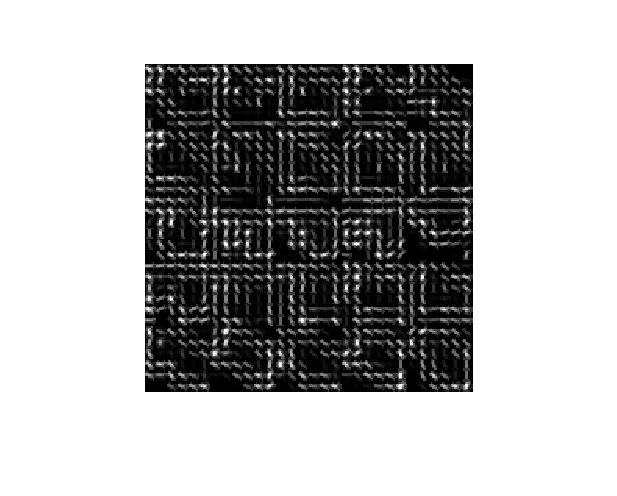
\includegraphics[trim={0cm 1cm 0cm 0cm},
  clip, width=0.45\linewidth]{figures/point_depth_hog.eps} }
\subfigure[]{
  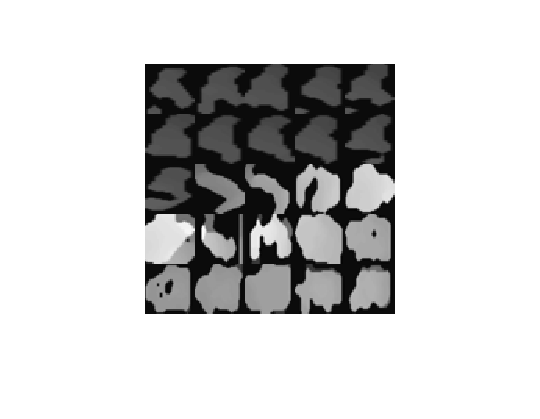
\includegraphics[width=0.5\linewidth,
  trim={0cm 1cm 0cm 0cm}, clip]{figures/other_depth_resize_32_denoise.eps} }
\subfigure[]{
  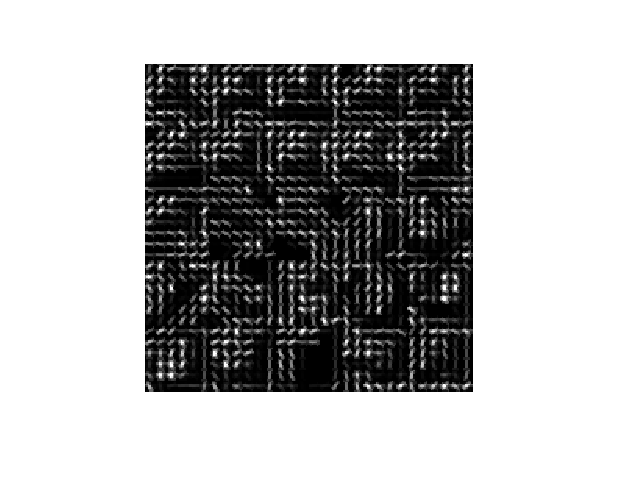
\includegraphics[trim={0cm 1cm 0cm 0cm},
  clip, width=0.45\linewidth]{figures/other_depth_hog.eps} }
\end{figure}

Radial Basis Function (RBF) kernel, use grid search to find best parameters, C =
0.03, $\gamma = 0.5$. Ratio between point pose and other poses is 27 : 73, so
the weight for $C_other$ and $C_point$ is 73 : 27. 

Test accuracy 92.6282\% (289/312) 2-class classfication


\section{Dictionary Learning}

\section{PCA and Sparse PCA}